\documentclass[12pt,a4paper]{amsart}
\usepackage[latin1]{inputenc}
\usepackage{graphicx}
\usepackage{amsmath}
\usepackage{amsfonts}
\usepackage{amssymb}
\usepackage{url}
\usepackage{cite}
%\usepackage{natbib}
\usepackage{colortbl}
\usepackage{tikz}
\usetikzlibrary{arrows,decorations.pathmorphing,fit,positioning}
\usepackage{algorithmic}

\title{Graphical model:\\ Lyric-based genre classification}
\author{David van Erkelens (10264019)\\ Sharon Gieske (6167667)\\ Elise Koster (5982448)}

\usepackage{fancyhdr}
\usepackage{booktabs}


% Set par indents to 0
\setlength{\parindent}{0cm}

% Set header for every page (except for first page)
\pagestyle{fancy}
\rhead[\small\textsc{David van Erkelens, Sharon Gieske, Elise Koster}]{\small\textsc{Proposal NLP Mini-project}}
\lhead{\thepage.}
\cfoot{}
\date{}

\begin{document}
\maketitle
\section{Topic distribution over genres using LDA}
To model topic distributions over genres, the dataset is split into the individual genres. Then, for each genre topic distributions per document are averaged, to provide a final topic distribution over genres.

\section{Plate Diagram}


\begin{figure}[htp]
  \centering
  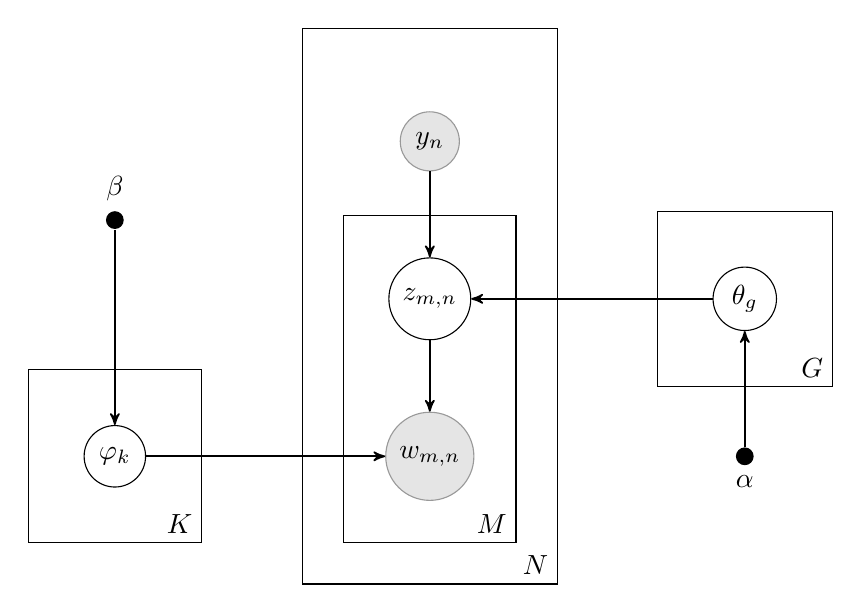
\begin{tikzpicture}
    [
      observed/.style={minimum size=15pt,circle,draw=gray!80,fill=gray!20},
      unobserved/.style={minimum size=15pt,circle,draw},
      hyper/.style={minimum size=1pt,circle,fill=black},
      post/.style={->,>=stealth',semithick},
    ]

    \node (w-j) [observed] at (0,0) {$w_{m,n}$};
    
    \node (z-j) [unobserved] at (0,2) {$z_{m,n}$};

    \node (y) [observed] at (0,4) {$y_n$};
    
    \node (z-prior) [unobserved] at (4,2) {$\theta_g$};
    
    \node (w-prior) [unobserved] at (-4,0) {$\varphi_k$};
    
    \node (z-hyper) [label=below:$\alpha$] at (4,0) {};
    
    \filldraw [black] (4,0) circle (3pt);
    
    \node (w-hyper) [label=above:$\beta$] at (-4,3) {};
    
    \filldraw [black] (-4,3) circle (3pt);
    
    \path
    (z-j) edge [post] (w-j)
    
    (z-hyper) edge [post] (z-prior)
    (z-prior) edge [post] (z-j)
    (y) edge [post] (z-j)


    (w-hyper) edge [post] (w-prior)
    
    (w-prior) edge [post] (w-j)
    ;

    \node [draw,fit=(w-j) (y), inner sep=30pt] (plate-context) {};
    \node [above left] at (plate-context.south east) {$N$};
    \node [draw, fit=(w-prior), inner sep=20pt] (plate-prior) {};
    \node [above left] at (plate-prior.south east) {$K$};
    \node [draw,fit=(w-j) (z-j), inner sep=15pt] (plate-token) {};
    \node [above left] at (plate-token.south east) {$M$};
    \node [draw, fit=(z-prior), inner sep=20pt] (plate-z-prior) {};
    \node [above left] at (plate-z-prior.south east) {$G$};

  \end{tikzpicture}
  \caption{Graphical model}
  \label{fig:graphical-model}
\end{figure}

\section{Derivation}
\begin{align}
P(w, z, \varphi, \theta | \alpha, \beta) &= P(\varphi | \beta)P(\theta | \alpha)P(z | \theta)P(w | \varphi, z)\\
P(\varphi | \beta) &= \prod\limits_{k=1}^K P(\varphi_k|\beta)\\
P(\theta | \alpha) &= \prod\limits_{g=1}^G P(\theta_g|\alpha)\\
P(z | \theta, y) &= \prod\limits_{i=1}^N \prod\limits_{j=1}^{M_i} P(z_{m,n}|\theta_g(z_{m,n}))P(y_i)\\
P(w | \varphi, z) &= \prod\limits_{i=1}^N \prod\limits_{j=1}^{M_i} P(w_{m,n}|\varphi_z(w_{m,n}))
\end{align}
\bibliography{../papers/bibliography}
\bibliographystyle{plain}

\end{document}